\asection{Ullman Algorithm}
\label{Ullman Algorithm}


\setlistdepth{9}

\newlist{myEnumerate}{enumerate}{9}
\setlist[myEnumerate,1]{label=(\arabic*)}
\setlist[myEnumerate,2]{label=(\Roman*)}
\setlist[myEnumerate,3]{label=(\Alph*)}
\setlist[myEnumerate,4]{label=(\roman*)}
\setlist[myEnumerate,5]{label=(\alph*)}
\setlist[myEnumerate,6]{label=(\arabic*)}
\setlist[myEnumerate,7]{label=(\Roman*)}
\setlist[myEnumerate,8]{label=(\Alph*)}
\setlist[myEnumerate,9]{label=(\roman*)}

\subsection{Background}
Subgraph ismorphis can be determined using a brute-force approach on the tree representation of a graph G{\tiny A}. Though this technique is effective, it is however not efficient because all the possible
permutation subgraphs of a graph G{\tiny A} are tested against the graph G{\tiny B} to determine if there are subgraphs in graph G{\tiny A} that are isomorphic to graph G{\tiny B}.The number of subgraphs of a graph G{\tiny A} increase at an exponential rate with every addition of a vertice Vn into the graph, thus the total number of subgraphs that are evaluated are  
	\begin{equation}
		ST = 2^{n/2}
	\end{equation} 
, where ST is the total
number of subgraphs and n the number if vertices in the graph G{\tiny A}.
The matching process is computationally expensive due to this very fact, that is the more vertices and there are in the graph G{\tiny A} the more expensive it becomes to detect the subgraph ismorphisms
because of the amount of subgraphs it has.

\subsection{Algorithm}
he Ullman algorithm was developed by J.R.Ullman and was published in his titled "An Algorithm for Subgraph Isomorphism"[1].The algorithm performs graph matching on an adjacency matrix representation of both the graphs, and uses the depth search first(DSF) recursicve approach to traverse through the graphs and perform
the graph matching process. The Ullman algorithm improves the effiency of the brute-force approach at detecting subgraph ismorphisms by deductively eleminating nodes in the tree that are in graph G{\tiny A}, but are not in graph G{\tiny B}, thus reducing the number of subgraphs that are matched against graph G{\tiny B}
to determine ismorphism.\newline\newline
The algorithm starts by building a starting adjacency matrix M0 using the two adjacency matrix representations of graphs G{\tiny A} and G{\tiny B} using the following procedure.
\begin{myEnumerate}
\item Construct a nxm matrix where n is the number of rows of graph G{\tiny B} and m is the number of colums of graph G{\tiny A}.
\item Set all the entries in the matrix to the value of 1.
\item Apply the following rule:
	Set the values in M0 to 0 for all M0ij where the degree of a vertice in graph G{\tiny A} at j is greater then the degree of the same vertice in graph G{\tiny B} .i.e. 
	\begin{equation}
		deg(Ai) < deg(Bj). 
	\end{equation}

\end{myEnumerate}
	A more formal representation of this rule is as follows
	\[
		f(x)= 
			\begin{cases}
				1,& \text{if } deg(Ai)\geq deg(Bj)\\ 
				0,              & \text{otherwise}\   \forall \text{i,j}
			\end{cases}
	\]
When the starting matrix has been constructed, we systematically permute matrices Md from the starting matrix M0 where d represents the depth of the generated matrix. The procedure of 
generating the permuted matrices follows a depth search first(DSF) recursicve approach where the stopping condition(leaf matrices) conform to the following form:
\begin{myEnumerate}
\item M contains only 0's and 1's.
\item There is exactly one 1 in each row.
\item Not more than one 1 in each colum.
\end{myEnumerate}

An demonstration of how the permutation matrices are generated is demonstrated in figure ~\ref{fig:permutationmatrix}.

\begin{figure}[H]
  \begin{center}
      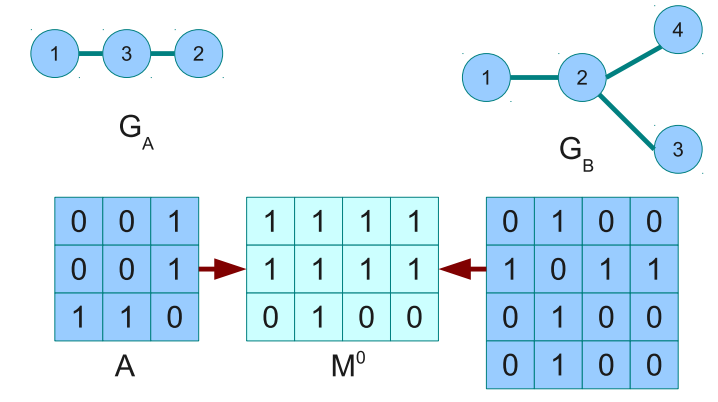
\includegraphics[width=0.65\textwidth]{permutationmatrix.png}
  \end{center}    
  \caption{Demonstation of how a permutation matrix is generated from two graphs} 
  \label{fig:permutationmatrix}
\end{figure} 

Once all the permutation matrices have been generated, each one of the matrices is matched with a graph C, that is obtained from the dot product of the permuted matrix and the graph G{\tiny A}.
The formula for calculating graph C is follows:
C=Mn(Mn . G{\tiny A})T, where
G{\tiny A} = input graph A
Mn = permutated matrix Mn in Md, obtained from the starting matrix M0
(Mn . G{\tiny A})T = the transpose of the dot product of the permutated matrix Mn and the graph G{\tiny A}.
If there is a single instance of the matrix C, that is calculated using some permutated matrix Mn obtained from the starting matrix M0, that is equal to matrix G{\tiny B}, then G{\tiny B} is isomorphic to G{\tiny A}. Thus G{\tiny B} is isomorphic to G{\tiny B} iff G{\tiny B}
  \begin{equation}	
	ij = 1 \rightarrow  Cij = 1 \forall i,j
  \end{equation} 


If non of the generated permutated matrices can statisfy this condition, then G{\tiny B} is not isomorphic to G{\tiny B}.
\newpage